\chapter{Beschreibung des Endproduktes}\label{cha:theoretical-background}
\section{Administrion}
\subsection{E-Mail und SMS}
\subsubsection{Massennachrichten}
Um regelmäßige Info- und Werbenachrichten auszusenden, bietet das Programm die Möglichkeit E-Mails oder SMS an alle Kunden zu versenden. Falls ein Kunde diese Nachrichten nicht mehr erhalten möchte, kann das der Benutzer bei dem einzelnen Kunden eintragen.
\subsubsection{E-Mail}
Wenn der Benutzer eine Massenemail versenden möchte, kann er einen Betreff und eine Nachricht eingeben, die nachher an alle Kunden gesendet wird. Als E-Mail-Adresse, wird die abgespeicherte Adresse des Kunden verwendet. Falls keine E-Mail-Adresse angegeben wurde, wird eine entsprechende Fehlermeldung angezeigt.

\begin{figure}[H]
\begin{center}
	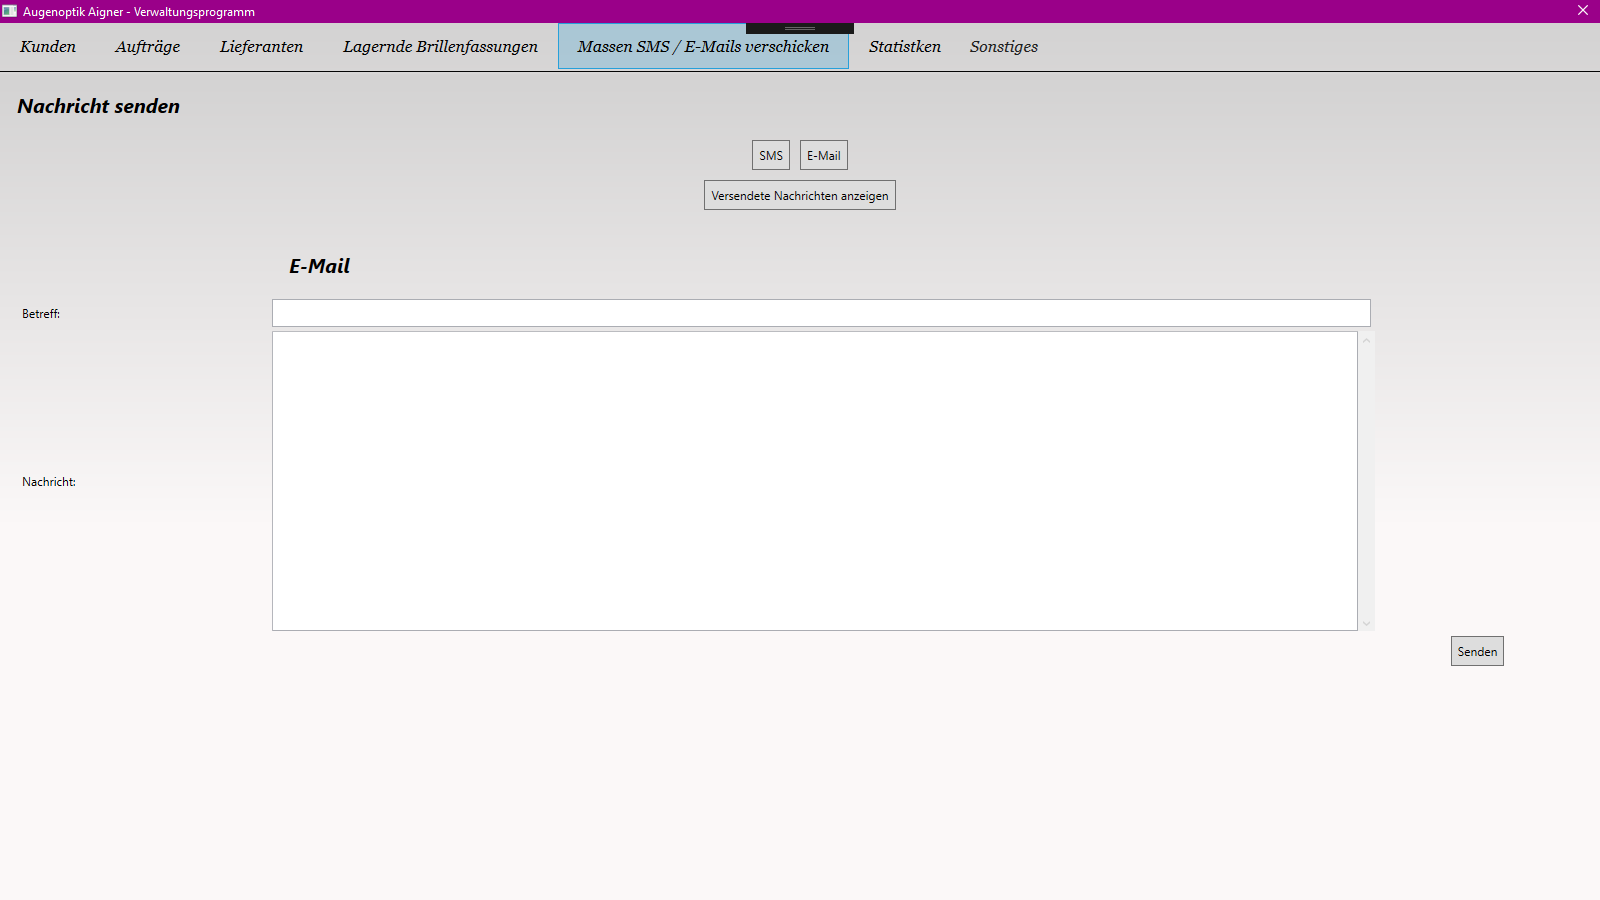
\includegraphics[scale=.25]{images/Massenemail.png}
\end{center}
	\caption{Screenshot der Massen E-Mails}
	\label{fig:sample}
\end{figure}
\underline{Technischer Hintergrund:}
\medskip
\linebreak
Es wird für jeden Kunden die gleiche Mail erstellt (Klasse MailMessage vom Namespace System.Net.Mail). Dieser Klasse werden Attribute, wie Sender, Empfänger, Betreff, Nachricht usw. übergeben und mittels eines SMTP-Clients versendet. (Klasse SmtpClient ebenfalls vom Namespace System.Net.Mail). Dem Smtp-Client müssen noch Eigenschaften wie Host, Port und natürlich die E-Mail-Adresse, von der die E-Mail weggeschickt werden soll sowie das Passwort für die E-Mail-Adresse angegeben werden. In diesem Fall wurde eine G-Mail-Adresse verwendet, die extra für diesen Zweck erstellt wurde.

\begin{lstlisting}
var message = new MailMessage();
message.To.Add(new MailAddress(item.Email));
message.From = new MailAddress("infodienst.augenoptikaigner@gmail.com");
message.Subject = this.Subject;
message.Body = this.Message;
this.Recipients.Add(new CustomRecipient() { Customer = item, Address = item.Email });

	using (var smtp = new SmtpClient())
    {
    	var credential = new NetworkCredential
		{
        	UserName = "infodienst.augenoptikaigner@gmail.com",
            Password = "7gnRwN4U"
        };
        smtp.Credentials = credential;
        smtp.Host = "smtp.gmail.com";
        smtp.Port = 587;
        smtp.EnableSsl = true;

        await smtp.SendMailAsync(message);
    }
        
\end{lstlisting}
\bigskip
Danach wird die gesendete Nachricht noch in die Datenbank abgespeichert, damit der Benutzer später alle gesendeten Nachrichten ansehen kann.

\subsubsection{SMS}
Zum Versenden der SMS wird der SMS-Dienst MessageBird verwendet (Referenz). Ähnlich wie beim Versenden einer E-Mail, gibt der Benutzer wieder eine Nachricht ein, allerdings kann er keine Betreff einfügen.
\begin{figure}[H]
\begin{center}
	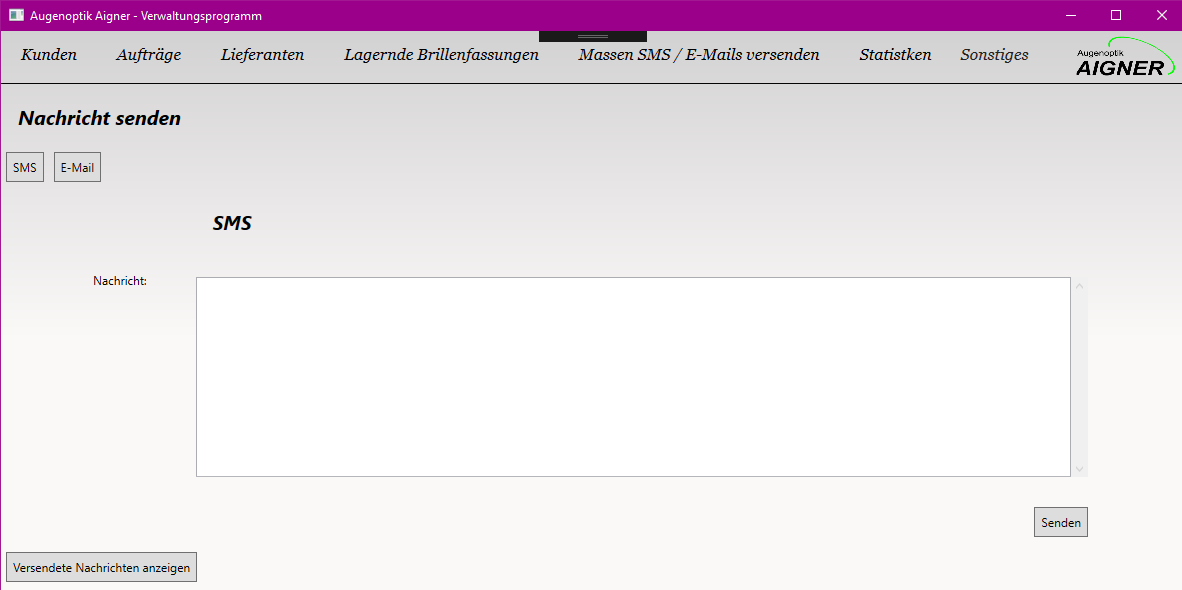
\includegraphics[scale=.25]{images/Massensms.png}
\end{center}
	\caption{Screenshot der Massen E-SMS}
	\label{fig:sample}
\end{figure}
Diese Nachricht wird dann an alle Kunden gesendet, außer jene, die keine Massennachricht mehr erhalten wollen. Als Telefonnummer wird standardmäßig die Telefonnummer 1 gewählt, außer diese ist nicht vorhanden, dann wird die Telefonnummer 2 gewählt. 
\newpage
\underline{Technischer Hintergrund:}
\linebreak
\linebreak 
Zum Senden einer Nachricht werden folgende Schritte benötigt:
\begin{lstlisting}
IProxyConfigurationInjector proxyConfigurationInjector = null;
Client client = Client.CreateDefault(AccessKey, proxyConfigurationInjector);
\end{lstlisting}
Und zum Versenden einer Nachricht:
\begin{lstlisting}
MessageBird.Objects.Message message = client.SendMessage("OptikAigner", this.Message, numbers);
\end{lstlisting}
Der AccessKey ist ein normaler String, der von MessageBird erstellt wird. Dabei kann jeder Benutzer von MessageBird mehrere AccessKeys haben, beispielsweise einen für Test-Nachrichten, die dann nicht versendet werden oder einen Key, mit dem dann echte SMS versendet werden.
Für jede Nachricht die versendet wird, wird das Guthaben auf MessageBird dementsprechend verringert. Sollte das Guthaben auslaufen, wird eine Fehlermeldung angezeigt.

\subsubsection{Einzelne Nachrichten}
Dieselben Vorgänge werden auch verwendet um einzelne Nachrichten zu versenden. Dazu muss der Benutzer auf die Detailseite einer Bestellung klicken und dann auf „Nachricht senden“. Standardmäßig wird ein Text eingefügt, der dem Kunden mitteilt, dass seine Bestellung nun abholbereit ist. Sollte dies nicht der Grund sein, warum eine Nachricht gesendet werden soll, kann der Benutzer die Nachricht natürlich auch verändern.
\begin{figure}[H]
\begin{center}
	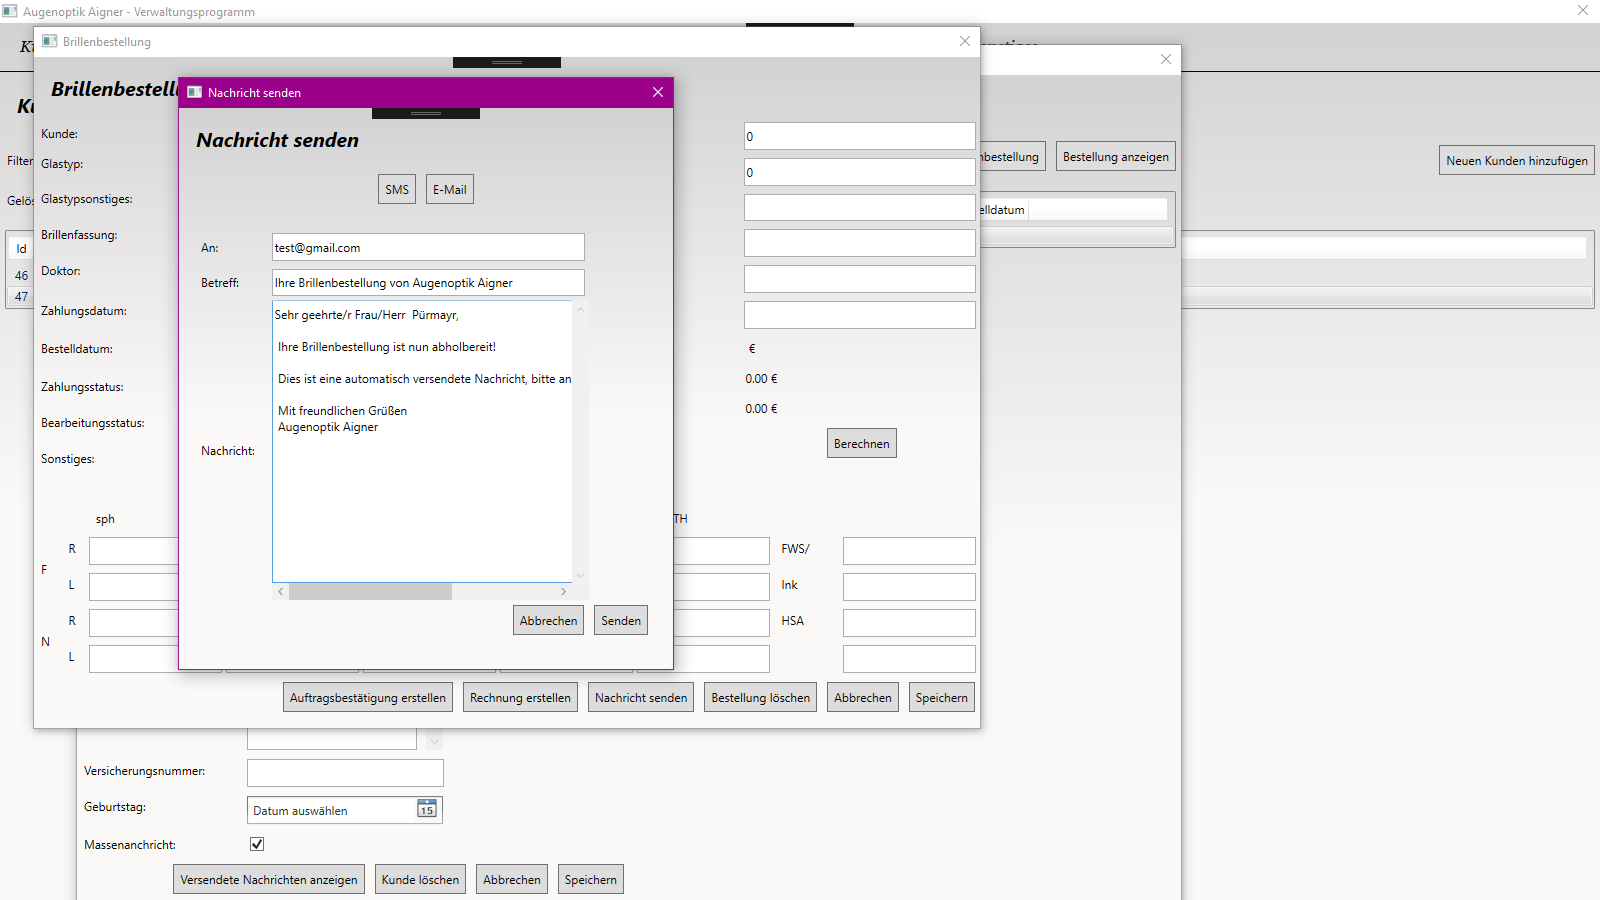
\includegraphics[scale=.25]{images/EinzelneNachricht.png}
\end{center}
	\caption{Screenshot der einzelnen Nachricht}
	\label{fig:sample}
\end{figure}
\subsubsection{Versendete Nachrichten}
Außerdem ist es möglich, alle Nachrichten, die vom System aus gesendet worden sind, anzuzeigen. Um nur Nachrichten anzuzeigen, die an einen bestimmten Kunden gesendet worden sind, muss der Benutzer auf die Detailseite eines Kunden klicken und dann die „Versendeten Nachrichten“ anzeigen. Falls der Benutzer alle Nachrichten sehen will, die er versendet hat, kann er unter dem Menüpunkt „Massen SMS /E-Mails verschicken“ auch alle bereits versendeten Nachrichten an alle Kunden sehen.
\begin{figure}[H]
\begin{center}
	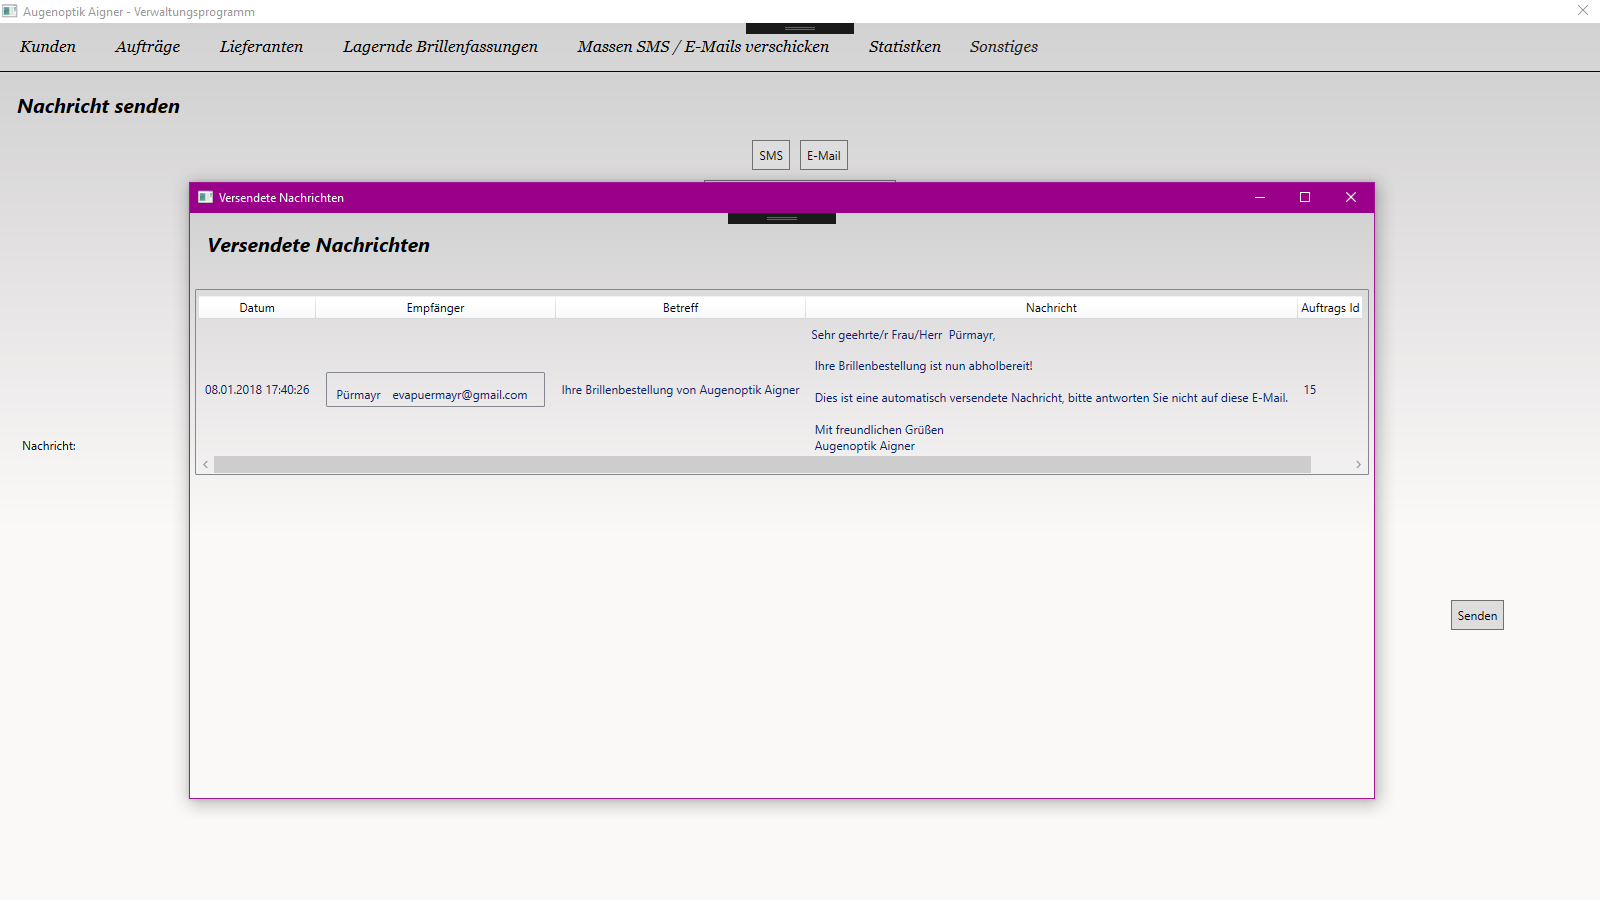
\includegraphics[scale=.25]{images/VersendeteNachrichten.png}
\end{center}
	\caption{Screenshot der versendeten Nachrichten}
	\label{fig:sample}
\end{figure}



\subsection{Statistiken}
Unter dem Menüpunkt ''Statistiken'' erhält der Benutzer eine Übersicht über alle verkauften Brillen und Kontaktlinsen. Dazu wird ein Liniendiagramm der verkauften Brillen/Kontaktlinsen von diesem Jahr und dem Jahr davor angezeigt. Damit eine Brille/Kontaktlinse in der Statistik mitberücksichtigt wird, muss ein Zahlungsdatum angegeben werden und der Bezahlungsstatus muss auf „Bezahlt“ gesetzt werden.
\begin{figure}[ht]
\begin{center}
	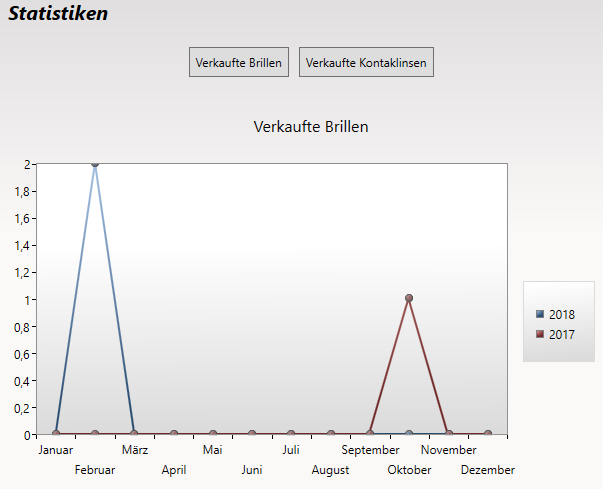
\includegraphics[scale=.25]{images/Statistiken.png}
\end{center}
	\caption{Screenshot der Statistiken}
	\label{fig:sample}
\end{figure}
\subsubsection{Technischer Hintergrund}
Zur Darstellung wurde das package System.Windows.Controls.DataVisualization.Toolkit 4.0.0 verwendet (hier Referenz einfügen). 
Dazu wird in dem .xaml File der Namespace angegeben: 
\begin{lstlisting}
<Page xmlns:toolkitCharting="clr-namespace:System.Windows.Controls
DataVisualization.Charting;assembly=System.Windows.Controls.DataVisualization
.Toolkit">
\end{lstlisting}
Um ein Liniendiagramm zu erzeugen:
\begin{lstlisting}
<toolkitCharting:Chart Title="{Binding Title}">
            <toolkitCharting:LineSeries Title="{Binding NewYear}"  DependentValueBinding="{Binding Value}" IndependentValueBinding="{Binding Key}" ItemsSource="{Binding NewValues}"/>
            <toolkitCharting:LineSeries Title="{Binding OldYear}"  DependentValueBinding="{Binding Value}" IndependentValueBinding="{Binding Key}" ItemsSource="{Binding OldValues}"/>
</toolkitCharting:Chart>
\end{lstlisting}
Dabei sind ''NewValues'' und ''OldValues'' vom Typ: 
\begin{lstlisting}
        public ObservableCollection<KeyValuePair<string, int>> NewValues { get; set; }
        public ObservableCollection<KeyValuePair<string, int>> OldValues { get; set; }
\end{lstlisting}
Die Daten werden mittels Linq(Referenz) erfasst.